\documentclass[12pt,a4paper]{article}
\usepackage{amsfonts}
\usepackage{amssymb}
\usepackage{graphicx}
\usepackage{bookmark}
\usepackage{hyperref}
\usepackage{enumitem}
\usepackage{changepage}
\usepackage{float}

\setlength{\parindent}{0em}

\graphicspath{{Images/}}

\begin{document}

\begin{titlepage}
  \begin{center}
    \begin{figure}[t]
      \centering
      
\includegraphics[width=350px]{logo.PNG}
     \end{figure}
     
     \textsc{\LARGE COS301 Group Task 2 \newline \newline Architectural Design\\[0.5cm] Specifications}
     
     \textbf{\newline Team Objective C} \\
     \begin{flushright} \large
      Diana Obo \emph{u13134885}\newline
      Kamogelo Tsipa \emph{u13010931}\newline
      Linda Zwane \emph{u14199468}\newline
      Melvin Zitha \emph{u12138747}\newline
      Minal Pramlall \emph{u13288157}\newline
      Rotondwa Siavhe \emph{u????????}\newline
       \end{flushright} 
      \vfill %whitespace
      
      Team Objective C Github: \href{https://github.com/ShockwaveZA/Objective-C-Team}{Github} page.\\
      \url{https://github.com/ShockwaveZA/Objective-C-Team}
      
      \vfill
      {\large Date:}
      \\
      {\large \today}
     \end{center}
    \end{titlepage}


\tableofcontents
\newpage
\section{External Interface Requirements}
\subsection{User interface}
When user or guest is navigating they should be able to see a search box where they must enter a location they want to travel to.Their current location should be visable on the map,see fig1 navigation.The points of interest will be shown in a list of different categoryies when you click on a category it will show you a more specific list of what you want,eg clicking on ATMs will show a list consisting of FNB,ABSA,Capitec and Nedebank,see fig2 points of interest.For the events module you be given two options either view all events or request to add an event,see fig3 events.The fitness module should allow the user to add their daily,weekly or monthly goals.It will show the stats of the day and green button if they have achieved their goal else a red button if they have not archieved their goal,see fig4 fitness.
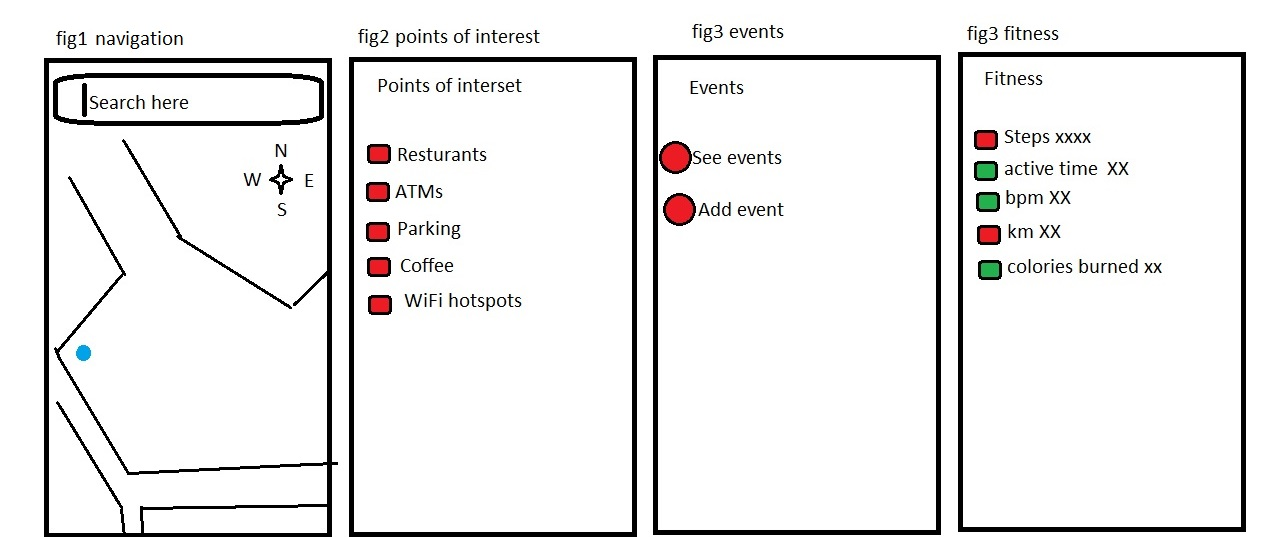
\includegraphics{userInterface}
\subsection{Hardware interface}
The NavUP system will be greatly dependant upon the user's/guest's device hardware system.Which could be either laptop,phone, tablet or phablet.
\subsection{Software interface}
The NavUP system will be greatly dependant upon the user's/guest's device operating system.Which could be either android or IOS.Web browsers could also be supported if there is also a web application created.The database will be a vital part of our system because it will get information from the user/guest and send it to google maps and then return the result of the search to the user via their operating system.The database will aslo be resposible for storing data to compute other places the user might be interested in.It will aslo store the data regarding to when and where events are taking place and also distance walked for the fitnes program. 
\subsection{Communications interface}
User/guset on the internet will use HTTP/HTTPS protocol.Adimin on the internet will use HTTP/HTTPS.The admin will also be using FTP
to put and get files from the server.
\section{Technology choices}
\subsection{Android SDK}
It has usefull developent tools which will be needed for the NavUP system.Android gives applications access to the location services compatable with the device via the classes in the android.location package.The LocationManager system service provides APIs to determine location and bearing of the device.
\subsection{WiFi}
WiFi is widely avaivable on campus for both students and guests.It will be used to allow users/guest to connect to the internet so they can make use of the the NavUP system.
\subsection{Database Server}
This ia a very impotant technology,because it will be used to store all the data such as the event dates and frequently visited place to help compute suggestions of simillar points of interest.
